%Correct the file name.
%X: book number
%Y: part number
%ZZZ: page number in three digits. So page 3 would be 003.

\documentclass[11pt]{amsbook}

\usepackage{../HBSuerDemir}	% ------------------------


\begin{document}

% ++++++++++++++++++++++++++++++++++++++
\hPage{feyzioglu/006}
% ++++++++++++++++++++++++++++++++++++++

\begin{enumerate}
		\item[2.]
			Show that \\
			$(R \cup S) \cup T = R \cup (S \cup T)$ and \\
			$(R \cap S) \cap T = R \cap (S \cap T)$. 

    	\item[3.]
    		Prove: $S \cap T = S$ if and only if $S \subseteq T$, and $S \subseteq T$ if and only if $S \cup T = T$.

    	\item[4.]
    		Prove the distributivity of union over intersection and of intersection over union:\\
    		$ R \cup (S \cap T) = (R \cup S) \cap (R \cup T),$\\
    		$ R \cap (S \cup T) = (R \cap S) \cup (R \cap T).$
    	
		\item[5.]
			Prove the deMorgan laws:\\
			$(S \cup T)^\mathsf{'} = S^\mathsf{'} \cap T^\mathsf{'}$ and $(S \cap T)^\mathsf{'} = S^\mathsf{'} \cup T^\mathsf{'}$\\ for any subsets S, T of a universal set U.

    	\item[6.]
    		Show that $T \setminus \varnothing = T$ and $ T 	\setminus T = \varnothing$ for any set T.

		\item[7.]
			Prove : $(S \setminus T) \cup (T \setminus S) = (S \cup T) \setminus (T \cap S).$ This set is called the \textit{symmetric difference of S and T}. It is denoted by $S \bigtriangleup T$.

		\item[8.]
			With the notation of Ex. 7, prove that\\
			$(R \bigtriangleup S) \bigtriangleup T = R \bigtriangleup (S \bigtriangleup T)$\\
			$S \bigtriangleup \varnothing = S $\\
			$S \bigtriangleup S = \varnothing$\\
			$S \bigtriangleup T = T \bigtriangleup S.$
			

		\item[9.]
			Let S and T be finite sets. Prove the following assertions.\\
			a) If $S \cap T = \varnothing$, then $ |S \cup T| = |S| + |T|$.\\
			b) $ |S \cup T| = |S| + |T| - |S \cap T|.$(Hint: $S \cup T = S \cup (T \setminus S).)$ 

		\item[10.]
			Find all subsets of $\varnothing , \{1\}, \{1, 2\}, \{1, 2, 3\}, \{1, 2, 3, 4\}$.
			
		\item[11.]
			Prove: if S is a finite set, then S has exactly $2^{|S|}$ subsets.
	
	\end{enumerate}


% =======================================================
\end{document}  

%==== templates ====

%==== environments ====

%\begin{figure}[htb]
%	\centering
%	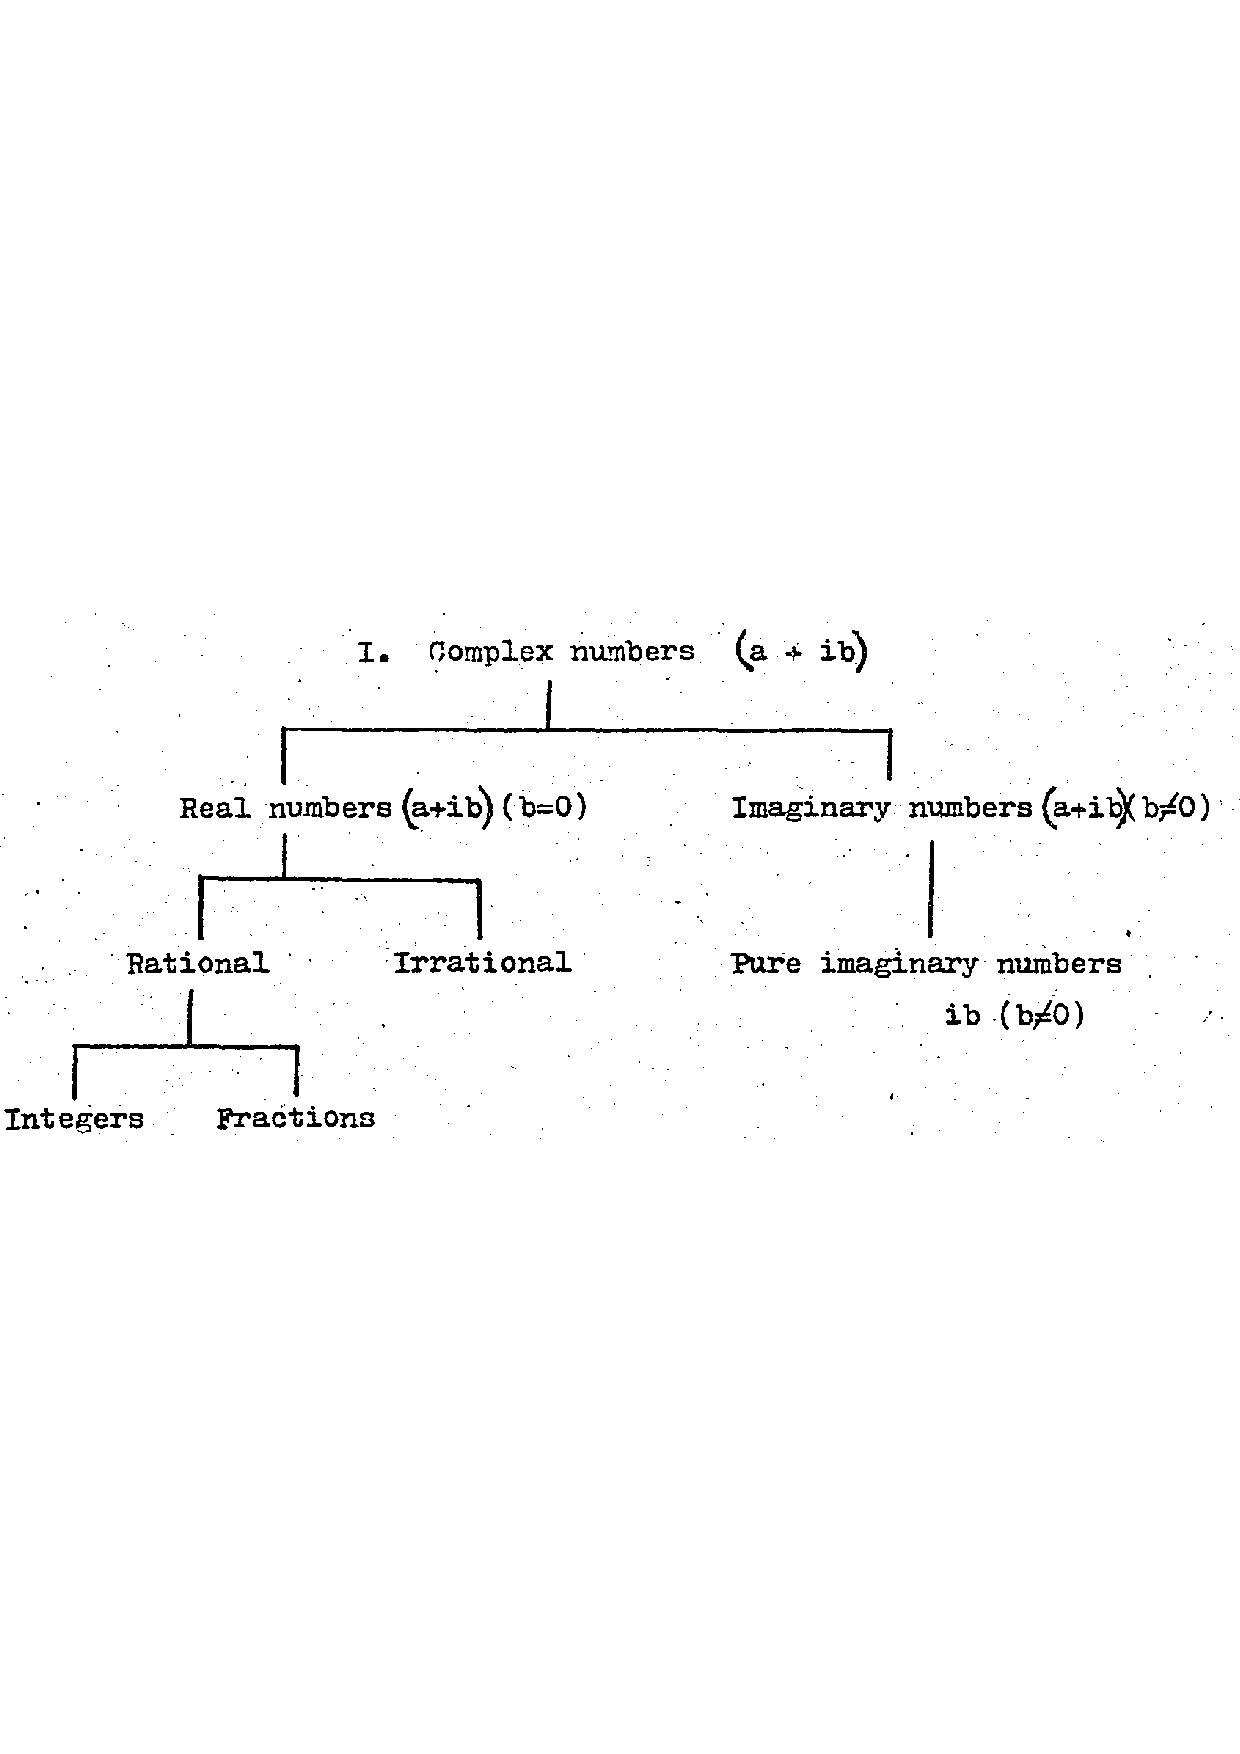
\includegraphics[width=0.9\textwidth]{images/SD-1-1p15A}
%	\caption{Classification of complex numbers}
%	\label{fig:classificationOfComplexNumbersA}
%\end{figure}

%\begin{center}
%\begin{tabular}{cc}
%\end{tabular}
%\end{center}

%\begin{exmp}
%\begin{hSolution}
%\end{hSolution}
%\end{exmp}

%\begin{hEnumerateAlpha}
%\end{hEnumerateAlpha}

%\begin{hEnumerateRoman}
%\end{hEnumerateRoman}

%$
%\begin{bmatrix}
%\end{bmatrix}
%$

%\frac{aaaa}{bbb}
%\frac{a_{n}}{b_{n}}
%\left( aaaa \right)
%\Longrightarrow

%\begin{multicols}{2}
%	bb
%\columnbreak
%	aa
%\end{multicols}
